% 编辑模板；build_report.py展开数值表至report_ready.tex。
\documentclass[UTF8,zihao=-4,fontset=fandol]{ctexart}
\usepackage[a4paper,left=22mm,right=20mm,top=23mm,bottom=21mm,headheight=15pt]{geometry}
\usepackage{fontspec,amsmath,amssymb,graphicx,booktabs,array,tabularx}
\usepackage[table]{xcolor}
\usepackage{float,caption,fancyhdr,enumitem,hyperref,attachfile2,fvextra}
\IfFileExists{/Users/john/Library/Fonts/NotoSerifCJKsc-Regular.otf}{
\setCJKmainfont[Path=/Users/john/Library/Fonts/,BoldFont=NotoSerifCJKsc-Bold.otf]{NotoSerifCJKsc-Regular.otf}
\setCJKsansfont[Path=/Users/john/Library/Fonts/,BoldFont=NotoSansCJKsc-Bold.otf]{NotoSansCJKsc-Regular.otf}}{}
\setmainfont[BoldFont=texgyretermes-bold.otf,ItalicFont=texgyretermes-italic.otf]{texgyretermes-regular.otf}
\setmonofont{lmmono10-regular.otf}
\hypersetup{colorlinks=true,linkcolor=black,urlcolor=blue!55!black,
  pdftitle={价量因子的研报复现与交易约束回测},pdfauthor={岳瀚阳}}
\captionsetup{font=small,labelfont=bf,labelsep=quad,skip=5pt}
\graphicspath{{figures/}}
\setlist{nosep,leftmargin=2em,topsep=4pt}
\renewcommand{\arraystretch}{1.25}
\setlength{\tabcolsep}{5pt}
\setlength{\parindent}{2em}
\setlength{\parskip}{3pt}
\setlength{\emergencystretch}{2em}
\linespread{1.23}
\setcounter{tocdepth}{1}
\ctexset{section={name={,},number=\chinese{section},format=\large\bfseries,beforeskip=12pt,afterskip=7pt},
 subsection={format=\normalsize\bfseries,beforeskip=9pt,afterskip=4pt}}
\pagestyle{fancy}\fancyhf{}
\fancyhead[L]{\small 岳瀚阳\quad 3230104443}
\fancyhead[R]{\small《量化投资》课程作业修订报告}
\fancyfoot[C]{\small\thepage}\renewcommand{\headrulewidth}{0.4pt}
\newcommand{\navfigure}[2]{\begin{figure}[H]\centering
\includegraphics[width=.97\linewidth,height=.415\textheight,keepaspectratio]{#1.pdf}
\caption{#2。上图为五组多头，下图为每腿100\%名义目标的费后理论多空组合。}\end{figure}}
\newcommand{\Trades}{12,157,512}
\newcommand{\Series}{588}
\newcommand{\CPVCSI}{8.05\%}
\newcommand{\CDPPCSI}{16.09\%}
\newcommand{\CPVAll}{13.14\%}
\newcommand{\CDPDPAll}{19.15\%}
\newcommand{\CandidateCount}{839}
\newcommand{\PrimaryMeanStocks}{453.4}
\newcommand{\ModelMeanStocks}{459.5}
\newcommand{\ModelRows}{215,483}
\newcommand{\XGBWeek}{14.35\%}
\newcommand{\XGBWeekSharpe}{1.83}
\newcommand{\XGBBiweek}{12.52\%}
\newcommand{\XGBBiweekSharpe}{1.70}
\newcommand{\XGBMonth}{17.89\%}
\newcommand{\XGBMonthSharpe}{2.48}

\begin{document}
\begin{titlepage}\thispagestyle{empty}\centering
\vspace*{-8mm}
\includegraphics[width=.60\linewidth]{char.png}\par
\vspace{8mm}
\includegraphics[width=.35\linewidth]{logo.png}\par
\vspace{8mm}{\LARGE\bfseries《量化投资》\par}
\vspace{4mm}{\Large\bfseries 价量因子的研报复现与交易约束回测\par}
\vspace{4mm}{\large 六因子、滚动合成与XGBoost实证\par}
\vspace{10mm}\renewcommand{\arraystretch}{1.7}
\begin{tabular}{rl}
姓\quad 名 & \underline{\makebox[68mm]{岳瀚阳}}\\
学\quad 号 & \underline{\makebox[68mm]{3230104443}}\\
学\quad 院 & \underline{\makebox[68mm]{管理学院}}\\
日\quad 期 & \underline{\makebox[68mm]{2026年11月14日}}\\
指导老师 & \underline{\makebox[68mm]{曾涛、彭旺}}\\
\end{tabular}
\vfill{\small 2016--2018年历史数据\quad ST、停复牌、实际涨跌停与官方复权版}
\end{titlepage}\setcounter{page}{2}

\begin{center}{\Large\bfseries 价量因子的研报复现与交易约束回测}\par
\vspace{3mm}岳瀚阳\quad 3230104443\end{center}
\noindent\textbf{摘要}\quad
本文逐篇核对四份本地研报，修正原\texttt{code2.py}及第一轮实现中的因子简化：聪明钱改为10日分钟池化，
CPV补入波动性和趋势并按阶段合成，CDPDP改为先分别标准化子项，普通振幅改为价格条件下的理想振幅，
另实现理想反转与CDPP。新增历史ST、日内停复牌、实际涨跌停价和官方复权因子均已接入。
本轮继续追溯原始研报，补齐理想振幅“剔除停牌及一字涨跌停、至少10个有效日”的细则；
上一版严格要求20日有效的结果冻结保留。本报告使用本轮重新生成的账本。
研究覆盖2016至2018年，完整检验动态中证500，并对全A价格相关因子进行补充核查。

自然月末、每腿100\%名义敞口且双边千三费用下，中证500的CPV与CDPP年化分别为\CPVCSI 和\CDPPCSI；
全A样本CPV与CDPDP$^{\prime}$分别为\CPVAll 和\CDPDPAll。
在2017年2月至2018年12月的共同样本外区间，XGBoost的5、10、20交易日策略年化分别为
\XGBWeek、\XGBBiweek、\XGBMonth，Sharpe分别为\XGBWeekSharpe、\XGBBiweekSharpe、\XGBMonthSharpe。
这些是有保证金融资和可借券假设的研究多空结果，报告同时列出每腿50\%的对照，不将增加敞口解释为因子改善。
公式配对实验也显示，忠实复现并不保证每个因子在当前样本都优于简化版本。

\noindent\textbf{关键词}\quad 价量因子；研报复现；历史交易状态；XGBoost；日频持仓回测
\vspace{3mm}\tableofcontents

\clearpage
\section{本轮重点因子的定义复核}
上一版仍存在遗漏，不能称为完全按照研报。20210924附录只给出了理想振幅的概要，
本轮进一步读取其引用的20200516原始报告第5页，发现“有效日”的定义包含两项关键限制：
剔除停牌和一字涨跌停，且窗口内少于10个有效日时才置空。
上一版要求20日全部有效，也未在历史窗口剔除一字板；只筛信号当天的交易状态不能代替历史窗口处理。

\begin{table}[H]\centering\small
\caption{表现较弱因子的再次核对结论}
\begin{tabularx}{\linewidth}{p{26mm}X}\toprule
因子 & 原文核对结论\\\midrule
理想振幅 & 高价端减低价端的公式和方向正确；历史有效日规则有遗漏，已修正并重跑。\\
聪明钱 & 10日池化、$|R|/V^{0.25}$、前20\%成交量及VWAP比值与2021附录一致。
2020原文有其他指数/对数版本，本轮未按收益选择其中最优版本。\\
CDPDP$^{\prime}$ & 相邻差分索引、同涨/同跌条件、20日均值和子项分别Z后相加均正确。
少于3对或零方差置0是原code2约定，原文未规定。\\
尾盘、偏度 & 来自原作业；四篇所给研报没有这两个定义，不应作为研报复现成败的证据。\\\bottomrule
\end{tabularx}\end{table}

新版理想振幅保持20交易日窗口，不向更早日期延长以凑满20个有效日。
令有效日数为$n$，要求$n\geq10$，每端取$k=\lfloor n/4\rfloor$日，因子为
\[
V=\frac1k\sum_{d\in\text{收盘价最高}k\text{日}}(H_d/L_d-1)
 -\frac1k\sum_{d\in\text{收盘价最低}k\text{日}}(H_d/L_d-1).
\]
舍入、并列价格和分钟首笔收益等细节未在研报公开，报告将其保留为实现约定。
固定3只股票、10日分钟数据的独立NumPy核对显示，聪明钱池化VWAP和四象限相关计算误差均小于$3\times10^{-15}$。
这验证算术实现，不证明与券商私有数据约定完全相同。

\clearpage
\section{课题具体说明与研报核对}
研究继续以原作业的分钟价量选股流程为基础，但将“修复回测程序”与“准确实现研报因子”分别核查。
此前实现解决了未来样本筛选、费用及净值问题，却仍沿用了原\texttt{code2.py}的简化因子，不能称为完整研报复现。
本轮先按原文确定公式和方向，再运行所有实验，没有根据当前回测收益挑选公式、方向或测试区间。

\begin{table}[H]\centering\small
\caption{四份研报的核对位置与本次处理}
\begin{tabularx}{\linewidth}{p{27mm}p{29mm}X}\toprule
来源 & 原文位置 & 核对结论与处理\\\midrule
东吴2020-02-23 & 第5、9、11--12页 & CPV包含均值、标准差和趋势。分别做指定处理后合成，均值子项不再冒充最终CPV。\\
东吴2021-03-01 & 第9--13、19页 & CDPP及四象限CDPDP均先处理子项；两项CDPDP$^{\prime}$为分别标准化后相加。\\
开源2021-09-24 & 第4、6--8页 & 聪明钱为10日分钟池；理想振幅按价格排序；理想反转按平均单笔金额排序；另核对160日低振幅动量及12期ICIR合成。\\
开源2022-12-18 & 第3--4、13--15页等 & 依赖主动/非主动及大中小单方向。当前新增数据没有这些字段，不以普通分钟量额冒充资金流因子。\\\bottomrule
\end{tabularx}\end{table}

本次六个主要研究和模型输入为聪明钱、完整CPV、CDPDP$^{\prime}$、理想振幅、理想反转、CDPP。
四象限CDPDP、长端动量、偏度、尾盘收益以及四个简化构造均另行输出，保留对照而非删去表现较弱的结果。
XGBoost是作业拓展；开源报告的滚动12期最大ICIR方法也单独移植，不能将两种合成方法混为一谈。

需要区分收益口径：研报多空是看好组与看空组之间的相对收益，并不要求多头在任何年份都赚钱。
例如东吴2020报告的2017、2018年多头端同样存在负收益；另有全A、指数成分和跨至2020/2021年的样本差异。
因此既不能把多头亏损直接当作因子无效，也不能要求当前短样本严格等于研报长样本收益。

\clearpage
\section{数据描述与交易状态处理}
\subsection{数据和证券身份}
分钟数据共731个交易日文件；日行情额外读取200交易日历史用于风格与160日窗口预热。
中证500读取\CandidateCount 只历史候选股票，信号日按当日历史成分选择。
上市60交易日过滤使用全历史首次正收盘报价日，未凭空补充精确上市日期。
全A补充检验限定于本地可识别A股，并按同样规则剔除ST及停牌样本。

\begin{table}[H]\centering\small
\caption{新增数据及其实际用途}
\begin{tabularx}{\linewidth}{p{27mm}X}\toprule
数据 & 连接键、字段与执行规则\\\midrule
ST情况 & 日期、代码；T日ST不进信号池。执行日新变ST只禁止增仓，不回头删除T日信号，减仓/回补仍可下单。\\
停复牌情况 & 日期、代码、suspend\_timing；空时段按全天停牌，有时段则检查09:30。午后停牌不阻止早盘成交，早盘停牌不借用稍后复牌价。\\
涨跌停价 & 日期、代码、up\_limit、down\_limit；开盘等于上限不买、等于下限不卖。上下限缺失、无效或与报价冲突时保守不成交，并导出异常清单。\\
复权因子 & 日期、代码、adj\_factor；连续价由原始价乘当日因子并以最早可得因子归一化。成交限制仍比较原始价。\\\bottomrule
\end{tabularx}\end{table}

统一证券身份贯通601313至601360、000022至001872的代码变更，避免复权与状态漏匹配或更名后遗留旧持仓。
其中000022/001872重复历史因子存在3位与4位精度差别，只容许半个旧精度单位的舍入误差，优先当前代码原始记录。
内部\texttt{SecuCode}表示连续证券身份，\texttt{TradingCode}记录当日实际交易代码。

覆盖检查包含预热期：中证500共781,109条股票日，其中ST为11,191条、停牌记录58,282条，
正常报价缺失实际限价或官方复权因子的条数均为0。全A对应3,336,704条股票日，同样无正常报价缺失限价或复权因子。
全A另有2条无效限价源记录及8条开盘超出所给上下限的记录，均单列而不强行撮合。

\subsection{时间对齐和不可成交处理}
T日收盘后生成信号，T+1的09:30执行，预测、IC及计划持有区间统一。
正常开盘价仍不保证涨跌停方向一定能成交；本轮按实际上下限采取保守订单规则，不使用任意4.9\%代理，
也不用当天最高/最低价判断早盘能否成交。已持有股票变ST，在下一个调仓日按新股票池下达退出单；
遇停牌、跌停或回补受阻，持仓保留并逐日重试，新调仓指令覆盖旧指令。
未知尾部行情沿用最近估值并披露，不用事后删除股票改善回撤。

\clearpage
\section{因子构造逻辑与公式}
\begin{table}[H]\centering\small
\caption{六个主要因子的研报定义及本次实现}
\begin{tabularx}{\linewidth}{p{28mm}X}\toprule
因子 & 实现方式\\\midrule
SmartMoney & 整个过去10交易日分钟池按$S_k=|r_k|/v_k^{0.25}$排序，取累计20\%成交量，
边界按比例切分；真实成交额构造$Q=\mathrm{VWAP}_{smart}/\mathrm{VWAP}_{all}$。
跨除权日统一连续价格及份额单位，不用每日Q的平均值替代。\\[2pt]
CPV & 20日日内价格-量相关系数的均值与标准差先市值中性化，再分别剔除反转、Z并相加，得到$D$。
相关系数对时间回归的趋势$B$剔除市值、反转、波动、换手；最终为$Z(D)+Z(B)$。\\[2pt]
CDPDP$^{\prime}$ & 对相邻价格差分的同涨、同跌子序列分别求日相关，20日聚合后各自市值中性化与Z，
定义$Z(\rho_{++})+Z(\rho_{--})$；四象限版本另加$-Z(\rho_{+-})-Z(\rho_{-+})$。\\[2pt]
IdealAmplitude & 日振幅为$H/L-1$。过去20日先剔除停牌及一字涨跌停；至少10个有效日。
按连续收盘价取最高/最低各25\%有效日，对应振幅均值相减，
并非普通$(H-L)/O$20日均值。\\[2pt]
IdealReversal & 按当日总成交额/总成交笔数求平均单笔成交金额。过去20日分高10日、低10日，
对应连续日收益分别加总后相减。\\[2pt]
CDPP & 对$\Delta P_t$与$P_{t+1}$，分别按$\Delta P_t$正负求条件相关。各自20日聚合、市值中性化、Z后，
采用正条件项减负条件项。\\\bottomrule
\end{tabularx}\end{table}

按原文因子方向，主要六因子均低值做多；模型分数高值做多。
每个截面先去极值，再进行该因子规定的处理，不把所有因子一律做行业和全部风格正交化。
零方差或不足3对的相关子序列恢复原\texttt{code2}的中性0约定，真正整日缺行情仍保持缺失。
这一原文未明确的实现约定有助于避免因低波动股票被连续剔除而造成流动性选择偏差，但也不能冒称研报明文规则。

以前共同样本日均约217只，本轮XGBoost共同输入日均约\ModelMeanStocks 只，共\ModelRows 条股票日。
样本恢复本身也是结果变化来源，不能把全部收益变化解释为公式修正。
有限风格变量不等于十个Barra风格因子的“纯净版”，缺少逐笔方向仍不能复制2022年大小单资金流模型。

\clearpage
\section{因子有效性分析}
\subsection{自然月末回测与股票池对照}
本节2016-01-29形成首个信号，2016-02-01开始计日收益，至2018-12-28，共711个日收益。
自然月信号取每月最后交易日，IC退出价为下一次月末信号的次日开盘，持有天数可变。
每个多头组独立等权；理论多空默认每腿100\%，合计200\%名义敞口，假定可借券及相应保证金融资。
每次买或卖费率各0.0015，两条腿分别按实际成交额扣费。

\begin{table}[H]\centering\small
\caption{中证500自然月末研究结果（实际交易状态约束）}
\setlength{\tabcolsep}{4pt}
\begin{tabular}{lrrrrrr}\toprule
因子 & 费前年化 & 费后年化 & Sharpe & 最大回撤 & 原始RankIC & 信号股数\\\midrule
SmartMoney & 10.01\% & 4.13\% & 0.59 & -8.69\% & -0.052 & 463 \\
CPV & 13.95\% & 8.05\% & 1.34 & -6.11\% & -0.080 & 453 \\
CDPDP-prime & 10.96\% & 6.68\% & 0.83 & -7.97\% & -0.087 & 453 \\
IdealAmplitude & 7.68\% & 2.10\% & 0.29 & -13.11\% & -0.052 & 467 \\
IdealReversal & 15.62\% & 9.73\% & 1.29 & -6.74\% & -0.076 & 453 \\
CDPP & 21.96\% & 16.09\% & 2.41 & -4.10\% & -0.094 & 453 \\
CDPDP-4 & 6.68\% & 3.11\% & 0.48 & -10.27\% & -0.053 & 453 \\
LowAmpMomentum & 6.73\% & 3.82\% & 0.57 & -8.64\% & 0.024 & 332 \\
Skewness & 13.24\% & 8.00\% & 1.19 & -8.29\% & -0.088 & 453 \\
TailReturn & 3.47\% & -1.44\% & -0.14 & -13.91\% & -0.006 & 453 \\
\bottomrule
\end{tabular}\end{table}

\begin{table}[H]\centering\small
\caption{相同公式与交易规则下的中证500、全A对照（费后）}
\setlength{\tabcolsep}{4pt}
\begin{tabular}{lrrrrrr}\toprule
因子 & 中证500年化 & Sharpe & 全A年化 & Sharpe & 全A回撤 & 全A股数\\\midrule
CPV & 8.05\% & 1.34 & 13.14\% & 2.91 & -2.17\% & 2755 \\
CDPP & 16.09\% & 2.41 & 16.59\% & 3.17 & -5.57\% & 2755 \\
CDPDP-prime & 6.68\% & 0.83 & 19.15\% & 2.21 & -7.86\% & 2755 \\
CDPDP-4 & 3.11\% & 0.48 & 12.60\% & 1.80 & -10.96\% & 2755 \\
\bottomrule
\end{tabular}\end{table}
全A补充只研究价格相关家族，不称为全A完整六因子模型。
表中加入了历史ST及停牌筛选，但样本仍短于研报，且上市日期和开盘队列数据不完整；
不能将年化差异当作复现全部数据条件的证明。原始IC仅作截面信息诊断，实际订单可因涨跌停或停牌而不成交。

\clearpage
\subsection{理想振幅遗漏修正后的独立对照}
下表固定资本、成本和成交约束，只改变定义及相应有效样本；全A补充直接使用日行情，
不依赖缺失的大小单字段。原始研报的有效日规则在回测前固定，未以收益决定保留哪一种版本。
\begin{table}[H]\centering\small
\caption{理想振幅：旧严格20日与原始研报有效日规则（费后）}
\setlength{\tabcolsep}{4pt}
\begin{tabular}{llrrrrr}\toprule
股票池 & 期限 & 旧年化 & 修订年化 & 修订Sharpe & 旧股数 & 修订股数\\\midrule
中证500 & 周频5日 & 0.48\% & 1.19\% & 0.17 & 455 & 468 \\
中证500 & 双周10日 & 7.24\% & 8.94\% & 0.99 & 455 & 468 \\
中证500 & 固定20日 & 11.00\% & 12.47\% & 1.36 & 454 & 467 \\
中证500 & 自然月末 & 2.14\% & 2.10\% & 0.29 & 453 & 467 \\
全A & 周频5日 & 15.22\% & 15.24\% & 2.05 & 2785 & 2874 \\
全A & 双周10日 & 19.71\% & 20.42\% & 2.81 & 2781 & 2870 \\
全A & 固定20日 & 17.89\% & 17.91\% & 2.43 & 2763 & 2853 \\
全A & 自然月末 & 13.12\% & 13.47\% & 2.07 & 2756 & 2846 \\
\bottomrule
\end{tabular}\end{table}

聪明钱及理想振幅的原始IC在各期限仍为负，与低值做多的方向相符。
费前、费后结果须同时查看，不能把扣费后偏弱直接归因于公式或反转方向。
\begin{table}[H]\centering\small
\caption{同一实现下的频率及费用影响}
\begin{tabular}{llrrr}\toprule
因子 & 期限 & 原始IC & 费前年化 & 费后年化\\\midrule
SmartMoney & 周频5日 & -0.043 & 20.06\% & 0.38\% \\
SmartMoney & 双周10日 & -0.060 & 22.68\% & 10.02\% \\
SmartMoney & 固定20日 & -0.067 & 19.69\% & 12.99\% \\
SmartMoney & 自然月末 & -0.051 & 10.01\% & 4.13\% \\
IdealAmplitude & 周频5日 & -0.044 & 15.97\% & 1.19\% \\
IdealAmplitude & 双周10日 & -0.061 & 19.24\% & 8.94\% \\
IdealAmplitude & 固定20日 & -0.077 & 18.89\% & 12.47\% \\
IdealAmplitude & 自然月末 & -0.042 & 7.68\% & 2.10\% \\
\bottomrule
\end{tabular}\end{table}
完整诊断另有“有效日放宽但不排一字板”及同样本自然月配对，均保存在
\path{results_code2_definition_audit/}。修正不能保证收益提高；自然月和固定20日的差异也原样保留。

\clearpage
\subsection{公式修订、成交约束与敞口的分离}
先将同一对新旧构造的有效股票日取交集，再使用完全相同日期、交易状态、名义敞口和费用。
因此下表比较的是构造流程（包括研报指定的分阶段处理），不混入不同股票池或旧版错误净值图。

\begin{table}[H]\centering\small
\caption{自然月末同样本新旧构造配对（费后）}
\begin{tabular}{lrrrrr}\toprule
因子 & 简化版年化 & 研报版年化 & 差异/百分点 & 简化Sharpe & 研报Sharpe\\\midrule
SmartMoney & 3.29\% & 4.13\% & +0.84 & 0.54 & 0.59 \\
CPV & 10.43\% & 8.05\% & -2.37 & 1.73 & 1.34 \\
CDPDP-prime & 7.07\% & 6.68\% & -0.39 & 0.89 & 0.83 \\
IdealAmplitude & 5.23\% & 2.24\% & -2.99 & 0.47 & 0.31 \\
\bottomrule
\end{tabular}\end{table}
\begin{figure}[H]\centering
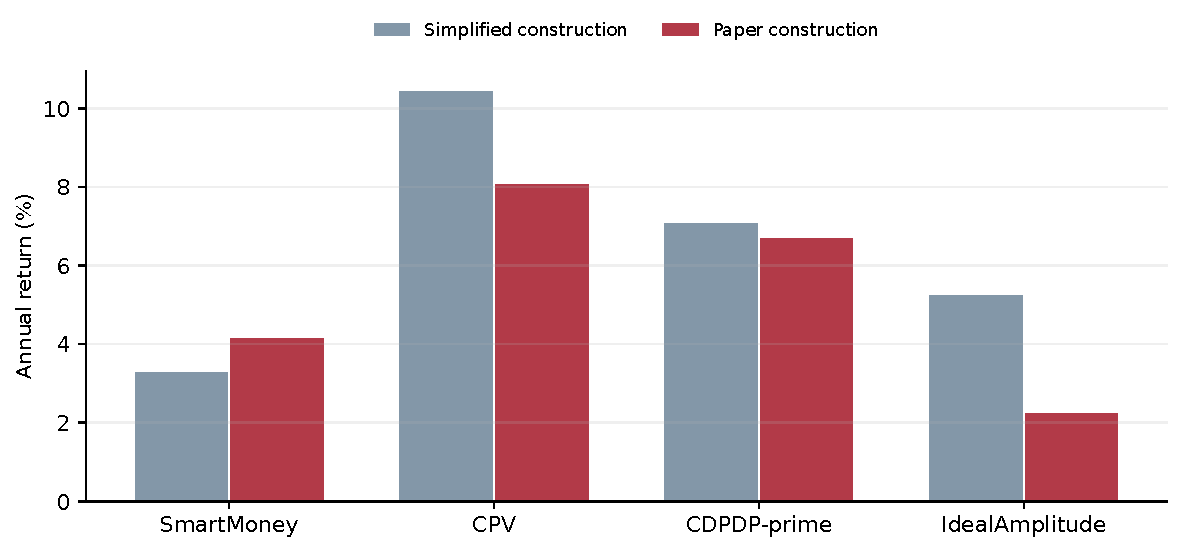
\includegraphics[width=.87\linewidth,height=.25\textheight,keepaspectratio]{paired.pdf}
\caption{配对结果原样展示，较忠实的公式并非在本样本中每项都更赚钱}
\end{figure}

\begin{table}[H]\centering\small
\caption{同一信号下的执行、费用及敞口敏感性（年化）}
\setlength{\tabcolsep}{4pt}
\begin{tabular}{lrrrr}\toprule
因子 & \shortstack{50\%每腿\\实际/费后} & \shortstack{100\%每腿\\实际/费后} & \shortstack{100\%每腿\\报价基准/费后} & \shortstack{100\%每腿\\实际/费前}\\\midrule
SmartMoney & 2.08\% & 4.13\% & 5.59\% & 10.01\% \\
CPV & 3.99\% & 8.05\% & 9.12\% & 13.95\% \\
CDPDP-prime & 3.36\% & 6.68\% & 8.29\% & 10.96\% \\
IdealAmplitude & 1.15\% & 2.10\% & 4.30\% & 7.68\% \\
\bottomrule
\end{tabular}\end{table}
报价基准仅移除开盘方向性价格及执行日ST增仓限制，保留信号日ST筛选和真正开盘停牌；
不能拿稍后复牌价冒充09:30价格。放松限制不保证收益上升，因为它会同时改变买入、退出与现金留存。
100\%每腿与50\%每腿收益不可直接比较；提高敞口的影响已单列，不当作因子能力提升。

\clearpage
\subsection{XGBoost与12期ICIR合成的共同样本检验}
共同样本为2017-02-03至2018-12-28信号，2017-02-06起468个日收益。
XGBoost分别预测5、10、20交易日的连续开盘收益减截面均值，每月使用过去12个月更新，
严格要求标签退出日在预测月首个交易日之前。参数固定为100棵树、深度5、学习率0.05、种子42。
未利用测试期调参或早停，三种期限共69个模型。

ICIR-12只使用已经实现的12个非重叠历史IC，求解最大ICIR方向，采用固定10\%对角收缩以稳定协方差逆。
这是将研报合成方法移植到当前六个可实现因子，未复制其含APM和大小单的原始六个输入。
固定20日期限初期历史不足12期时按现金等待，不用未来数据补足。

\begin{table}[H]\centering\footnotesize
\caption{共同样本费后理论多空（每腿100\%名义目标）}
\setlength{\tabcolsep}{4pt}\renewcommand{\arraystretch}{1.05}
\begin{tabular}{llrrrrr}\toprule
期限 & 因子/模型 & IC & 年化 & Sharpe & 最大回撤 & 信号股数\\\midrule
周频5日 & SmartMoney & -0.047 & 0.20\% & 0.06 & -7.56\% & 459 \\
 & CPV & -0.047 & 8.60\% & 1.29 & -6.78\% & 459 \\
 & CDPDP-prime & -0.025 & 3.27\% & 0.41 & -8.77\% & 459 \\
 & IdealAmplitude & -0.043 & 3.83\% & 0.42 & -8.73\% & 459 \\
 & IdealReversal & -0.032 & 0.33\% & 0.08 & -14.37\% & 459 \\
 & CDPP & -0.051 & 16.84\% & 2.63 & -3.51\% & 459 \\
 & ICIR-12 & 0.051 & 9.22\% & 1.33 & -5.71\% & 459 \\
\rowcolor{blue!7}
 & XGBoost & 0.051 & 14.35\% & 1.83 & -5.44\% & 459 \\
\midrule
双周10日 & SmartMoney & -0.057 & 2.66\% & 0.39 & -5.45\% & 458 \\
 & CPV & -0.054 & 11.14\% & 1.66 & -5.39\% & 458 \\
 & CDPDP-prime & -0.032 & 4.12\% & 0.51 & -8.66\% & 458 \\
 & IdealAmplitude & -0.055 & 4.66\% & 0.52 & -8.90\% & 458 \\
 & IdealReversal & -0.037 & 2.37\% & 0.33 & -7.64\% & 458 \\
 & CDPP & -0.061 & 12.47\% & 1.98 & -3.54\% & 458 \\
 & ICIR-12 & 0.054 & 10.35\% & 1.47 & -5.26\% & 458 \\
\rowcolor{blue!7}
 & XGBoost & 0.067 & 12.52\% & 1.70 & -4.29\% & 458 \\
\midrule
固定20日 & SmartMoney & -0.052 & 3.39\% & 0.53 & -7.36\% & 458 \\
 & CPV & -0.067 & 15.69\% & 2.43 & -4.61\% & 458 \\
 & CDPDP-prime & -0.042 & 4.12\% & 0.52 & -7.44\% & 458 \\
 & IdealAmplitude & -0.060 & 4.94\% & 0.57 & -12.72\% & 458 \\
 & IdealReversal & -0.040 & 6.01\% & 0.80 & -5.81\% & 458 \\
 & CDPP & -0.060 & 10.57\% & 1.66 & -3.58\% & 458 \\
 & ICIR-12 & 0.056 & 8.23\% & 1.14 & -5.15\% & 458 \\
\rowcolor{blue!7}
 & XGBoost & 0.073 & 17.89\% & 2.48 & -4.17\% & 458 \\
\midrule
\bottomrule
\end{tabular}\end{table}
所有案例都按同一完整输入股票日及调仓日历评估，保留真实未成交和延迟退出。
固定20日不是自然月；自然月因子研究与模型期限分开列示，避免用20日预测结果声称检验了任意自然月持仓。

\clearpage
\subsection{模型的资本口径与净值}
\begin{table}[H]\centering\small
\caption{XGBoost实际约束下的每腿100\%与50\%费后对照}
\setlength{\tabcolsep}{4pt}
\begin{tabular}{lrrrrrr}\toprule
期限 & 100\%年化 & Sharpe & 回撤 & 50\%年化 & Sharpe & 回撤\\\midrule
周频5日 & 14.35\% & 1.83 & -5.44\% & 7.02\% & 1.83 & -2.75\% \\
双周10日 & 12.52\% & 1.70 & -4.29\% & 6.13\% & 1.70 & -2.19\% \\
固定20日 & 17.89\% & 2.48 & -4.17\% & 8.63\% & 2.48 & -2.09\% \\
\bottomrule
\end{tabular}\end{table}
持仓、现金和成交费用均独立计算，未把100\%每腿收益机械除以二充作50\%结果。
价格波动、受阻订单和费用会使实际多空敞口偏离目标，理论多空并非始终市场中性。

\navfigure{model_biweekly}{XGBoost双周10交易日共同样本回测}
日净值由现金加多头市值减空头市值形成。净值图、几何年化、日收益Sharpe及日频回撤来自同一序列，
初始净值1计入回撤高水位。样本末日尝试平仓，受阻持仓仍保留，不能当作已经全部变现的收益。

\clearpage
\begin{figure}[H]\centering
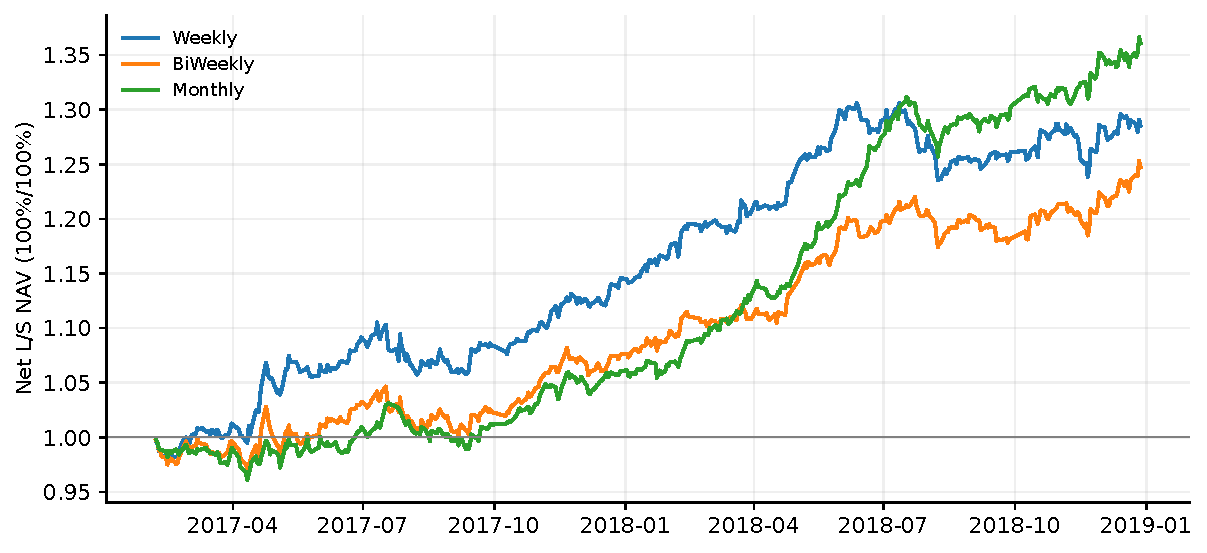
\includegraphics[width=.95\linewidth,height=.31\textheight,keepaspectratio]{model_horizons.pdf}
\caption{三个模型期限的费后理论多空净值（实际状态约束）}
\end{figure}
\section{因子思考与改进}
第一轮表现不理想既有构造简化，也有实验口径变化。均值代替完整CPV、日均Q代替池化Q、原始相关相加代替逐项Z，
与样本压缩、4.9\%代理及50\%每腿敞口混在一起，无法据此评价研报因子。
本轮把这些层面分别列出，并保留表现较差的理想振幅、尾盘及简化对照，不以收益目标反向选择公式。

新增状态数据使ST与涨跌停无需再估计，但并未补齐开盘订单队列、借券供应与资金规模冲击。
开盘等于限价一律视为对应方向受阻是保守规则，不能声称精确还原排队成交。
源数据存在少量特殊复牌/恢复上市日的开盘与上下限冲突，已导出并禁止其可疑订单，未删掉未来表现不佳的股票。
下一步若研究实盘容量，应补充逐笔与借券数据；若研究完整Barra纯净版，应补齐风格暴露，而不是继续改动当前测试收益。

\section{结论}
本次已按原文修正主要因子，并将新增ST、停复牌、实际涨跌停价及官方复权因子接入信号、成交和估值。
中证500自然月CPV、CDPP费后年化分别为\CPVCSI、\CDPPCSI；全A补充的CPV、CDPDP$^{\prime}$分别为\CPVAll、\CDPDPAll。
共同样本XGBoost的5、10、20交易日年化分别为\XGBWeek、\XGBBiweek、\XGBMonth，
但资本、借券和执行假设应与数字一起阅读。

研报逻辑复现不等于保证每项因子更高收益，也不等于完整复制其数据条件。
本轮结果更适合说明：正确公式、可得样本、交易状态和资本口径必须同时固定后，才能进行有意义的因子与模型比较。

\clearpage
\section{代码输出与可复现性}
完整主实验包含32个单因子/对照案例、8个配对案例及24个共同样本案例；另有6个全A价格相关案例。
本轮额外有28个理想振幅定义/股票池/频率案例，包含同样本自然月配对。
每个案例保留信号分组、IC、实际成交、现金和持仓日账本及净值图，适用案例另输出费前账本。
本次对\Series 条费后组合账本和\Trades 笔成交逐项核对现金、成本、净值及绩效，58项测试通过。

\begin{Verbatim}[fontsize=\small,frame=single,breaklines=true]
python code2_new.py --with-xgboost
python audit/full_a_price_factors.py
python audit/constraints_sensitivity.py
python audit/recheck_factor_definitions.py
python -m unittest discover -s tests -p 'test_code2*.py' -v
python report_definitions/build_report.py
\end{Verbatim}
主结果位于\path{results_code2_definitions/}，全A价格相关补充位于\path{results_research_all_a_constraints/}。
本轮理想振幅的定义与全A对照位于\path{results_code2_definition_audit/}。
\texttt{trading\_data\_diagnostics.json}保存新增数据覆盖、代码映射、异常限价及输入文件签名；
\texttt{daily\_market.parquet}保存实际执行掩码、状态及官方复权价格。
\texttt{missing\_limits.csv}与\texttt{inconsistent\_limits.csv}提供可复查清单，
\texttt{FinalPositions}与\texttt{StalePositionDays}标明尾部风险，不为获得平滑曲线而清空受阻股票。

\subsection*{完整源码附件}
PDF内嵌四个源码；压缩包另附测试、运行日志与表格源数据。
\begin{itemize}
\item \attachfile[icon=Paperclip,mimetype=text/plain]{source/code2_new.py}\quad 主入口与持仓账本。
\item \attachfile[icon=Paperclip,mimetype=text/plain]{source/code2_research.py}\quad 研报因子与ICIR合成。
\item \attachfile[icon=Paperclip,mimetype=text/plain]{source/code2_xgboost.py}\quad 按月滚动XGBoost。
\item \attachfile[icon=Paperclip,mimetype=text/plain]{source/code2_trading_data.py}\quad 新增交易数据与代码贯通。
\end{itemize}

\begin{thebibliography}{9}\footnotesize
\setlength{\itemsep}{1pt}\setlength{\parskip}{0pt}\linespread{1.05}\selectfont
\bibitem{r1} 东吴证券．高频价量相关性，意想不到的选股因子．2020-02-23，第5、9、11--12、17页。
\bibitem{r2} 东吴证券．CPV因子错位版，价量自相关性中蕴藏的选股信息．2021-03-01，第9--13、19页。
\bibitem{r3} 开源证券．独家量价因子的高频测试．2021-09-24，第4、6--8页。
\bibitem{r4} 开源证券．大小单资金流alpha探究2.0：变量精筛与高频测算．2022-12-18。
\bibitem{r5} 开源证券．振幅因子的隐藏结构．2020-05-16，第5--7页。
\bibitem{r6} 开源证券．聪明钱因子模型的2.0版本．2020-02-09，第3、5--6、9页。
\bibitem{data} 课程本地日/分钟行情、历史成分及新增ST、停复牌、涨跌停价、复权因子文件；本次运行配置和验证记录。
\end{thebibliography}

\appendix
\clearpage
\section{研报因子自然月末净值图}
\navfigure{HF_SmartMoney_MonthEnd}{SmartMoney自然月末回测}
\vfill
\navfigure{HF_CPV_MonthEnd}{CPV自然月末回测}
\clearpage
\navfigure{HF_CDPDP_MonthEnd}{CDPDP-prime自然月末回测}
\vfill
\navfigure{HF_IdealAmplitude_MonthEnd}{IdealAmplitude自然月末回测}
\clearpage
\navfigure{HF_IdealReversal_MonthEnd}{IdealReversal自然月末回测}
\vfill
\navfigure{HF_CDPP_MonthEnd}{CDPP自然月末回测}
\clearpage\section{理想振幅的全A补充净值}
\navfigure{AllA_IdealAmplitude_MonthEnd}{理想振幅全A自然月末回测}
\vfill
\navfigure{AllA_IdealAmplitude_BiWeekly}{理想振幅全A双周10日回测}

\end{document}
